
\documentclass{beamer}
\usepackage[utf8]{inputenc}
\usetheme{focus} % Use the Focus theme supplied with the template
% Add option [numbering=none] to disable the footer progress bar
% Add option [numbering=fullbar] to show the footer progress bar as always full with a slide count

% Uncomment to enable the ice-blue theme
\definecolor{main}{RGB}{50, 97, 133}
\definecolor{background}{RGB}{240, 247, 255}

%------------------------------------------------

\usepackage{booktabs} % Required for better table rules
\usepackage{subcaption}
\usepackage{multirow}

%----------------------------------------------------------------------------------------
%	 TITLE SLIDE 
%----------------------------------------------------------------------------------------

\title{Word Count Problem \& \\Cross Correlation Calculation}

\subtitle{MPI Implementation}

\author{Filipe Pires | 85122 | filipesnetopires@ua.pt \\ João Alegria | 85048 | joao.p@ua.pt}

\institute{University of Aveiro, DETI}

\date{\today}

%------------------------------------------------

\begin{document}

%------------------------------------------------

\begin{frame}
	\maketitle % Automatically created using the information in the commands above
\end{frame}

%----------------------------------------------------------------------------------------
%	 WORD COUNT
%----------------------------------------------------------------------------------------

\begin{frame}{Multi-Thread to MPI Mapping}
	Given that a multi-thread solution was already implemented, the team's efforts were focused on mapping the it to the MPI environment.
	The required mapping was:
	\begin{itemize}
		\item The previous central entity(monitor) was translated to a dispatcher that is responsible for the same functionalities and is implemented in a predefined process created by the MPI platform.
		\item The dispatcher is responsible for keeping track of files to process, provide data chunk when requested, stored partial results and print final results.
		\item The previous thread workers are now implemented as process supported by the MPI platform.
		\item There logic keeps the same, but now they wait for a data chunk to process, sending the obtained results to the dispatcher.
	\end{itemize}
\end{frame}

%------------------------------------------------

\begin{frame}{Word Count Entity Interaction}
	\begin{figure}
		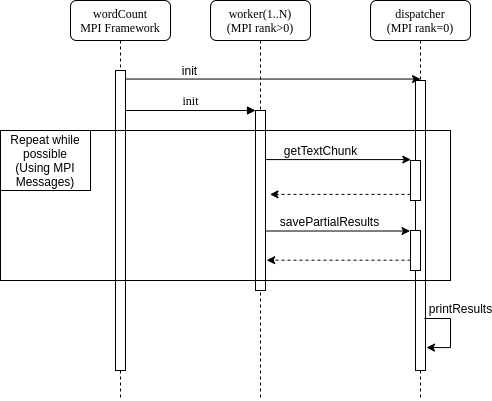
\includegraphics[width=0.7\linewidth]{wordCountInteraction.png}
		\caption{Entity Interactions}
		\label{wordInteraction}
	\end{figure}
\end{frame}

%------------------------------------------------

%----------------------------------------------------------------------------------------
%	 CROSS CORRELATION CALCULATION
%----------------------------------------------------------------------------------------

% \begin{frame}{Cross Correlation Problem: Multi-Thread Mapping}
% 	Once again, our task was to map a single-threaded implementation of the solution for this second problem, previously developed by us, to a multi-threaded
% 	version of such implementation.
% 	The required mapping was:
% 	\begin{itemize}
% 		\item A shared memory space would keep track of the files to be processed.
% 		\item Each worker thread would ask the shared memory for the values of a signal and a specific $\tau$, calculate the cross correlation and return the results to the shared memory.
% 		\item The shared memory would manage the files' content internally, enabling the distribution of the same signals but with different $\tau$ values.
% 		\item The shared memory would keep track of all received results, enabling the program to write the results in the end of each file or to print them to the console.
% 	\end{itemize}
% \end{frame}

%------------------------------------------------

\begin{frame}{Cross Correlation Entity Interaction}
	\begin{figure}
		\includegraphics[width=0.7\linewidth]{crossCorrelationInteraction.png}
		\caption{Entity Interactions}
		\label{crossInteraction}
	\end{figure}
\end{frame}

%------------------------------------------------

%----------------------------------------------------------------------------------------
%	 RESULTS TABLE
%----------------------------------------------------------------------------------------

\begin{frame}{Results}
	As expected, the more worker processes the user deploys, the faster it delivers the results.

	By analyzing the table below, it is not difficult to see an inverse relation between the number of threads and the execution times.

	\tiny {
		\begin{table}[]
			\begin{tabular}{|l|l|l|l|l|l|l|l|l|l|}
				\hline
				\multicolumn{2}{|l|}{\multirow{3}{*}{}}                          & \multicolumn{8}{l|}{Average Execution Time (s)}                                                                                                   \\ \cline{3-10}
				\multicolumn{2}{|l|}{}                                           & \multicolumn{4}{l|}{Problem 1}                  & \multicolumn{4}{l|}{Problem 2}                                                                  \\ \cline{3-10}
				\multicolumn{2}{|l|}{}                                           & text1                                           & text2                          & text3 & text4 & sigVal1 & sigVal2 & sigVal3 & sigVal4          \\ \hline
				\multicolumn{1}{|c|}{\multirow{3}{*}{\begin{tabular}[c]{@{}c@{}}\# of\\ Threads\end{tabular}}} & 1                                               & 0.004                          & 0.038 & 0.010 & 0.026   & 0.006   & 0.132   & 2.408   & 36.985 \\ \cline{2-10}
				\multicolumn{1}{|c|}{}                                           & 2                                               & 0.005                          & 0.020 & 0.008 & 0.015   & 0.006   & 0.067   & 1.764   & 25.453 \\ \cline{2-10}
				\multicolumn{1}{|c|}{}                                           & 4                                               & 0.002                          & 0.019 & 0.006 & 0.013   & 0.005   & 0.0657  & 1.334   & 21.481 \\ \hline
			\end{tabular}
			\caption*{Table: average execution time of running the programs 10 times for each input file and for each different number of worker threads.}
		\end{table}
	}


\end{frame}

%------------------------------------------------

%----------------------------------------------------------------------------------------
%	 CONCLUSIONS
%----------------------------------------------------------------------------------------

\begin{frame}{Conclusions}

	The results of implementing a multi-process version using the MPI library for the different problems proved to be a good option to the multi-thread approach. By carefully orchestrating the worker processes, we were able to speed up our solutions up to 2 times. In fact this achievement can be greater if there are more CPU cores and therefore supports a higher number of processes. A conclusion we made during tests was that if the number of processes used exceed the number of possible threads in the system, the application can suffer in performance, possibly due to the action of exchanging different processes in and out the CPU, which can be costly.

	For future work, one possible improvement would be do adopt different computation approaches, such as using multidimensional techniques for the cross-correlation calculation.

\end{frame}

\end{document}
